\section*{Atividade aula 7}

\begin{enumerate}
	\item \textbf{Utilizando uma linguagem de programação, codifique um somatório para somar os valores as posições de cor verde da matriz. Os valores dessa posições devem ser informados pelo usuário.}
	\begin{figure}[H]
		\centering
		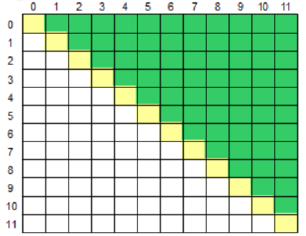
\includegraphics{7_1}
	\end{figure}
	\lstinputlisting{../src/7_1.cpp}
	\verb|[12:24]| - A soma dos valores nas posições verdes (acima da diagonal principal) é acumulada sempre que o índice das linhas for menor que o índice das colunas.

	\pagebreak
	\item \textbf{Utilizando uma linguagem de programação, codifique um somatório para somar os valores as posições de cor verde da matriz. Os valores dessa posições devem ser informados pelo usuário.}
	\begin{figure}[H]
		\centering
		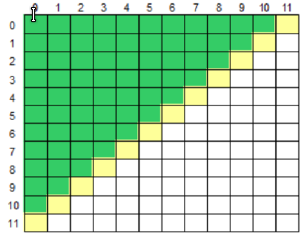
\includegraphics{7_2}
	\end{figure}
	\lstinputlisting{../src/7_2.cpp}
	\verb|[12:24]| - A soma dos valores nas posições verdes (acima da diagonal secundária) é acumulada sempre que a soma do índice das linhas com o índice das colunas for menor que o tamanho da matriz $-1$.
	
	\pagebreak
	\item \textbf{Utilizando uma linguagem de programação, codifique um somatório para somar os valores as posições de cor verde da matriz. Os valores dessa posições devem ser informados pelo usuário.}
	\begin{figure}[H]
		\centering
		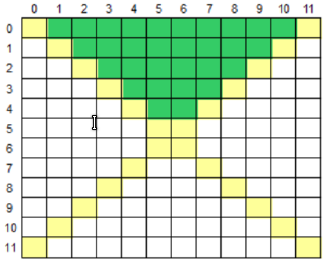
\includegraphics{7_3}
	\end{figure}
	\lstinputlisting{../src/7_3.cpp}
	\verb|[12:24]| - A soma dos valores nas posições verdes (acima de ambas as diagonais) é acumulada sempre que os índices forem parte da interseção entre os valores acima da diagonal principal e acima da diagonal secundária.
	
	\pagebreak
	\item \textbf{Utilizando uma linguagem de programação, codifique um somatório para somar os valores as posições de cor verde da matriz. Os valores dessa posições devem ser informados pelo usuário.}
	\begin{figure}[H]
		\centering
		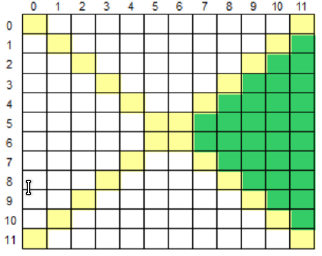
\includegraphics{7_4}
	\end{figure}
	\lstinputlisting{../src/7_4.cpp}
	\verb|[12:24]| - A soma dos valores nas posições verdes (entre ambas as diagonais, pela direita) é acumulada sempre que os índices forem parte da interseção entre os valores acima da diagonal principal e abaixo da diagonal secundária.
	
	\pagebreak
	\item \textbf{Utilizando uma linguagem de programação, codifique um somatório para somar os valores as posições de cor verde da matriz. Os valores dessa posições devem ser informados pelo usuário.}
	\begin{figure}[H]
		\centering
		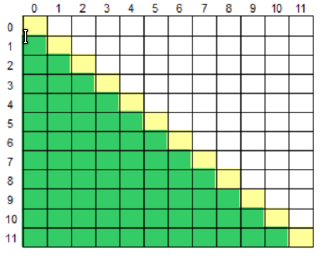
\includegraphics{7_5}
	\end{figure}
	\lstinputlisting{../src/7_5.cpp}
	\verb|[12:24]| - A soma dos valores nas posições verdes (abaixo da diagonal principal) é acumulada sempre que os índices das linhas for maior que o índice das colunas.
	
	\pagebreak
	\item \textbf{Utilizando uma linguagem de programação, codifique um somatório para somar os valores as posições de cor verde da matriz. Os valores dessa posições devem ser informados pelo usuário.}
	\begin{figure}[H]
		\centering
		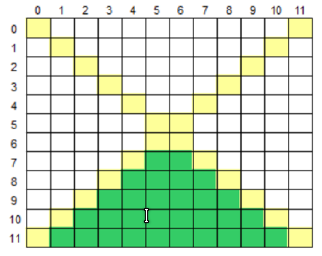
\includegraphics{7_6}
	\end{figure}
	\lstinputlisting{../src/7_6.cpp}
	\verb|[12:24]| - A soma dos valores nas posições verdes (abaixo de ambas as diagonais) é acumulada sempre que os índices forem parte da interseção entre os valores abaixo da diagonal principal e abaixo da diagonal secundária.
	
	\pagebreak
	\item \textbf{Utilizando uma linguagem de programação, codifique um somatório para somar os valores as posições de cor verde da matriz. Os valores dessa posições devem ser informados pelo usuário.}
	\begin{figure}[H]
		\centering
		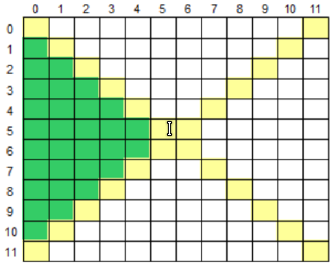
\includegraphics{7_7}
	\end{figure}
	\lstinputlisting{../src/7_7.cpp}
	\verb|[12:24]| - A soma dos valores nas posições verdes (entre ambas as diagonais, pela esquerda) é acumulada sempre que os índices forem parte da interseção entre os valores abaixo da diagonal principal e acima da diagonal secundária.
	
	\pagebreak
	\item \textbf{Utilizando uma linguagem de programação, codifique um somatório para somar os valores as posições de cor verde da matriz. Os valores dessa posições devem ser informados pelo usuário.}
	\begin{figure}[H]
		\centering
		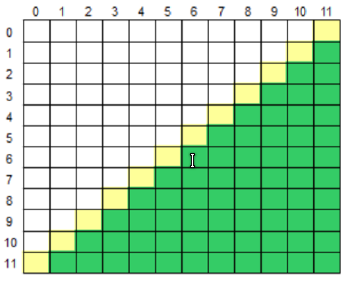
\includegraphics{7_8}
	\end{figure}
	\lstinputlisting{../src/7_8.cpp}
	\verb|[12:24]| - A soma dos valores nas posições verdes (abaixo da diagonal secundária) é acumulada sempre que a soma do índice das linhas com o índice das colunas for maior que o tamanho da matriz $-1$.
	
\end{enumerate}